\documentclass[journal,12pt,twocolumn]{IEEEtran}

\usepackage{setspace}
\usepackage{gensymb}

\singlespacing


\usepackage[cmex10]{amsmath}

\usepackage{amsthm}

\usepackage{mathrsfs}
\usepackage{txfonts}
\usepackage{stfloats}
\usepackage{bm}
\usepackage{cite}
\usepackage{cases}
\usepackage{subfig}

\usepackage{longtable}
\usepackage{multirow}

\usepackage{enumitem}
\usepackage{mathtools}
\usepackage{steinmetz}
\usepackage{tikz}
\usepackage{circuitikz}
\usepackage{verbatim}
\usepackage{tfrupee}
\usepackage[breaklinks=true]{hyperref}

\usepackage{tkz-euclide}

\usetikzlibrary{calc,math}
\usepackage{listings}
    \usepackage{color}                                            %%
    \usepackage{array}                                            %%
    \usepackage{longtable}                                        %%
    \usepackage{calc}                                             %%
    \usepackage{multirow}                                         %%
    \usepackage{hhline}                                           %%
    \usepackage{ifthen}                                           %%
    \usepackage{lscape}     
\usepackage{multicol}
\usepackage{chngcntr}

\DeclareMathOperator*{\Res}{Res}

\renewcommand\thesection{\arabic{section}}
\renewcommand\thesubsection{\thesection.\arabic{subsection}}
\renewcommand\thesubsubsection{\thesubsection.\arabic{subsubsection}}

\renewcommand\thesectiondis{\arabic{section}}
\renewcommand\thesubsectiondis{\thesectiondis.\arabic{subsection}}
\renewcommand\thesubsubsectiondis{\thesubsectiondis.\arabic{subsubsection}}


\hyphenation{op-tical net-works semi-conduc-tor}
\def\inputGnumericTable{}                                 %%

\lstset{
%language=C,
frame=single, 
breaklines=true,
columns=fullflexible
}
\begin{document}


\newtheorem{theorem}{Theorem}[section]
\newtheorem{problem}{Problem}
\newtheorem{proposition}{Proposition}[section]
\newtheorem{lemma}{Lemma}[section]
\newtheorem{corollary}[theorem]{Corollary}
\newtheorem{example}{Example}[section]
\newtheorem{definition}[problem]{Definition}

\newcommand{\BEQA}{\begin{eqnarray}}
\newcommand{\EEQA}{\end{eqnarray}}
\newcommand{\define}{\stackrel{\triangle}{=}}
\bibliographystyle{IEEEtran}
\providecommand{\mbf}{\mathbf}
\providecommand{\pr}[1]{\ensuremath{\Pr\left(#1\right)}}
\providecommand{\qfunc}[1]{\ensuremath{Q\left(#1\right)}}
\providecommand{\sbrak}[1]{\ensuremath{{}\left[#1\right]}}
\providecommand{\lsbrak}[1]{\ensuremath{{}\left[#1\right.}}
\providecommand{\rsbrak}[1]{\ensuremath{{}\left.#1\right]}}
\providecommand{\brak}[1]{\ensuremath{\left(#1\right)}}
\providecommand{\lbrak}[1]{\ensuremath{\left(#1\right.}}
\providecommand{\rbrak}[1]{\ensuremath{\left.#1\right)}}
\providecommand{\cbrak}[1]{\ensuremath{\left\{#1\right\}}}
\providecommand{\lcbrak}[1]{\ensuremath{\left\{#1\right.}}
\providecommand{\rcbrak}[1]{\ensuremath{\left.#1\right\}}}
\theoremstyle{remark}
\newtheorem{rem}{Remark}
\newcommand{\sgn}{\mathop{\mathrm{sgn}}}
\providecommand{\abs}[1]{\left\vert#1\right\vert}
\providecommand{\res}[1]{\Res\displaylimits_{#1}} 
\providecommand{\norm}[1]{\left\lVert#1\right\rVert}
%\providecommand{\norm}[1]{\lVert#1\rVert}
\providecommand{\mtx}[1]{\mathbf{#1}}
\providecommand{\mean}[1]{E\left[ #1 \right]}
\providecommand{\fourier}{\overset{\mathcal{F}}{ \rightleftharpoons}}
%\providecommand{\hilbert}{\overset{\mathcal{H}}{ \rightleftharpoons}}
\providecommand{\system}{\overset{\mathcal{H}}{ \longleftrightarrow}}
	%\newcommand{\solution}[2]{\textbf{Solution:}{#1}}
\newcommand{\solution}{\noindent \textbf{Solution: }}
\newcommand{\cosec}{\,\text{cosec}\,}
\providecommand{\dec}[2]{\ensuremath{\overset{#1}{\underset{#2}{\gtrless}}}}
\newcommand{\myvec}[1]{\ensuremath{\begin{pmatrix}#1\end{pmatrix}}}
\newcommand{\mydet}[1]{\ensuremath{\begin{vmatrix}#1\end{vmatrix}}}
\numberwithin{equation}{subsection}
\makeatletter
\@addtoreset{figure}{problem}
\makeatother
\let\StandardTheFigure\thefigure
\let\vec\mathbf
\renewcommand{\thefigure}{\theproblem}
\def\putbox#1#2#3{\makebox[0in][l]{\makebox[#1][l]{}\raisebox{\baselineskip}[0in][0in]{\raisebox{#2}[0in][0in]{#3}}}}
     \def\rightbox#1{\makebox[0in][r]{#1}}
     \def\centbox#1{\makebox[0in]{#1}}
     \def\topbox#1{\raisebox{-\baselineskip}[0in][0in]{#1}}
     \def\midbox#1{\raisebox{-0.5\baselineskip}[0in][0in]{#1}}
\vspace{3cm}
\title{ Matrix Theory : Assignment 3 }
\author{Ritesh Kumar \\ Roll no. : EE20RESCH11005 }
\maketitle
\newpage
\bigskip
\renewcommand{\thefigure}{\theenumi}
\renewcommand{\thetable}{\theenumi}
\begin{abstract}
This problem is to demonstrate the way to prove the triangles are congruent and to prove a triangle as isosceles using matrix algebra.
\end{abstract}

\section{Problem}
ABC is a triangle in which altitudes BE and CF to sides AC and AB are equal. Show that 
\begin{enumerate}
	\item $\triangle$ABC $\cong$ $\triangle$ACF 
%	\item AB = AC  i.e $\triangle$ABC is an isosceles triangle.
\end{enumerate}
\section{Solution}
\subsection{part 1}
Let consider we have a triangle $\triangle$ABC. There are two altitudes BE and CF being  drawn from the vertices B and C respectively. \newline
 In $\triangle$ABE, taking inner product of sides  AE and EB we can write :
\begin{align}
\left( \vec{A-E} \right)^T \left( \vec{E - B} \right) = \norm{\vec{A - E}} \norm{\vec{ E - B}} \text{cosAEB}
\end{align}
\begin{align}
\implies \text{cosAEB} = \frac{\left( \vec{A-E} \right)^T  \left( \vec{E - B } \right)}{\norm{\vec{A - E}} \norm{\vec{E - B}}}
\end{align}
In $\triangle$ACF, taking inner product of sides AF and FC :
\begin{align}
\left( \vec{A-F} \right)^T \left( \vec{F - C} \right) = \norm{\vec{A - F}} \norm{\vec{ F - C}} \text{cosAFC}
\end{align}

\begin{align}
\implies \text{cosAFC} = \frac{\left( \vec{A-F} \right)^T  \left( \vec{F - C } \right)}{\norm{\vec{A - F}} \norm{\vec{F - C}}}
\end{align}
 In triangle $\triangle$ABC, 
 \begin{align}
 \text{cosAFC} = \text{cosAEB} \left( \text{CF} \perp \text{AB} \hspace{2pt} \& \hspace{2pt} \text{BE} \perp \text{AC}\right)    
 \end{align}
 \begin{figure}[htb!]	
 	\centering	
 	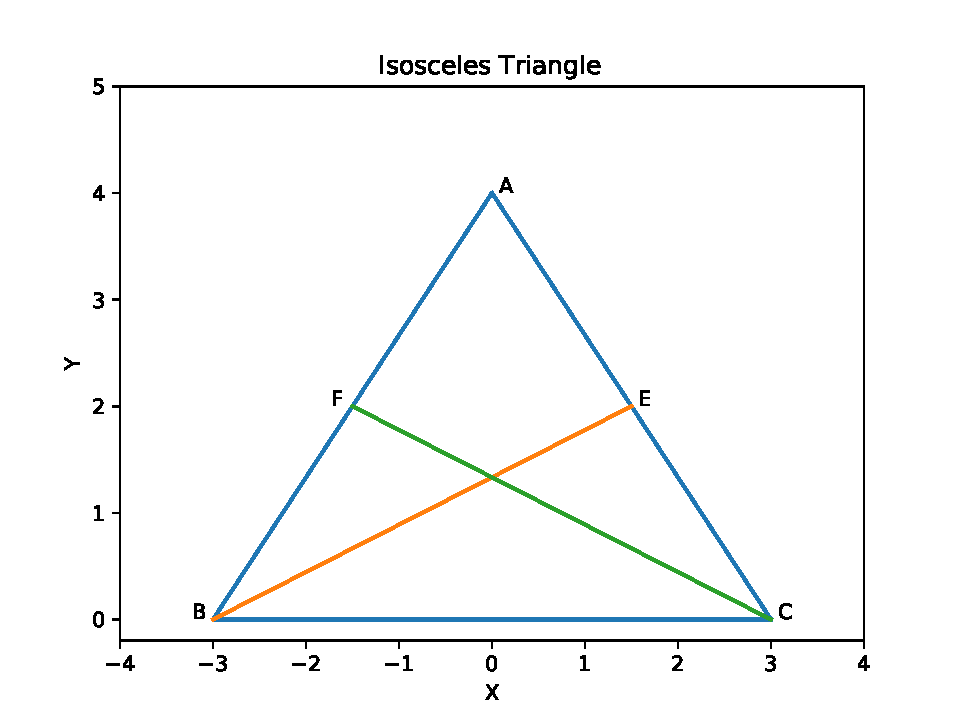
\includegraphics[width=.50\textwidth, height=.30\textheight]{Figure_1.pdf}	
 	\caption{Isosceles triangle}
 	\label{fig1}	
 \end{figure}

Given,  
\begin{align}
\norm{\vec{E - B}} = \norm{\vec{F - C}} \label{eq7}
\end{align}
\begin{align}
\angle FAC = \angle EAB \left( \text{Common angle}\right) \label{eq1.8}
\end{align}
 We know that if the two angles of triangles are equal then the third angle will also be equal.Hence,
 \begin{align}
 \angle FCA = \angle EBA  \label{eq1.9}
 \end{align}
   Hence by ASA (  Angle - Side - Angle ) We can say that , $\triangle$ABC $\cong$ $\triangle$ACF.
% \begin{align}
%\frac{\left( \vec{A-E} \right)^T  \left( \vec{E - B } \right)}{\norm{\vec{A - E}} \norm{\vec{E - B}}} =  \frac{\left( \vec{A-F} \right)^T  \left( \vec{F - C } \right)}{\norm{\vec{A - F}} \norm{\vec{F - C}}}
%\end{align}
%%
%\begin{align}
%\frac{ \left( \vec{A-E} \right)^T  \left( \vec{E - B } \right)}{\left ( \vec{A - E} \right )^T \left ( \vec{A - E} \right ) }  =   \frac{ \left( \vec{A-F} \right)^T  \left( \vec{F - C } \right)} { \left ( \vec{A - F}  \right )^T \left ( \vec{A - F} \right ) }
%\end{align}

% \begin{align}
%\frac{\left( \vec{A-E} \right)^T  \left( \vec{E - B } \right)}{\norm{\vec{A - E}}} =  \frac{\left( \vec{A-F} \right)^T  \left( \vec{F - C } \right)}{\norm{\vec{A - F}}}
%\end{align}
%
%\begin{align}
%\frac{ \left( \vec{E - B } \right)}{ \left ( \vec{A - E} \right ) } =  \frac{ \left( \vec{F - C } \right)} { \left ( \vec{A - F} \right ) }
%\end{align}
%Taking norms both side,
% 
%\begin{align}
%\frac{ \norm{ \vec{E - B }} }{ \norm{ \vec{A - E}} } =  \frac{ \norm{\vec{F - C }}}{\norm{\vec{A - F}}} \label{eq10}
%\end{align}

 


% Using \ref{eq7} in \ref{eq10} we get :
% 
% 
% 
% \begin{align}
% \norm{ \vec{A - E}} =  \norm{\vec{A - F}} \label{eq11}
% \end{align}
% Now, we have
% \begin{align}
%\norm{ \vec{A - E}} =  \norm{\vec{A - F}} \label{eq12} \left( \text{ we got the result} \right)
%\end{align}
% \begin{align}
%  \norm{ \vec{C - F}} =  \norm{\vec{B - E}}  \left( \text{given} \right) 
% \end{align}
% since BE $\perp$ AC and CF $\perp$ AB  , hence we have,
%  \begin{align}
%   \text{cos}BEA =  \text{cos}CFA \left( \text{ 90\degree } \right)   \label{eq1.14}
% \end{align}  
%   
% 
%  Hence by SAS ( Side - Angle - Side ) We can say that , $\triangle$ABC $\cong$ $\triangle$ACF  
%  
%  
  
  
 
% \subsection{part 2} 
%  In $\triangle$ABC we can have :
%
%\begin{align}
% \text{cosABC} = \frac{\left( \vec{A-B} \right)^T  \left( \vec{B - C } \right)}{\norm{\vec{A - B}} \norm{\vec{B - C}}} \label{eq2.1}
%\end{align}
%And,
%\begin{align}
% \text{cosACB} = \frac{\left( \vec{A-C} \right)^T  \left( \vec{C - B } \right)}{\norm{\vec{A - C}} \norm{\vec{C - B}}} \label{eq2.2}
%\end{align}
%  Since,
%   \begin{align}
%  \norm{ \vec{A - C}} =  \norm{\vec{A - B}}  \left(  \triangle \text{AEB} \cong \triangle \text{ AFC}  \right) \label{eq2.3}
%  \end{align}
% 
%   \begin{align}
%  \norm{ \vec{B - C}} =  \norm{\vec{C - B}}  \label{eq2.4}
%  \end{align}
%  
% Divindg \ref{eq2.1} to \ref{eq2.2}, and we get :
% 
% \begin{align}
% \frac{\text{cosABC}}{\text{cosACB}} = \frac{\left( \vec{A-B} \right)^T  \left( \vec{B - C } \right)}{\left( \vec{A-C} \right)^T  \left( \vec{C - B } \right)} \label{eq2.5}
% \end{align}
% By multiplying right hand side of equation \ref{eq2.5} by $\frac{\left( \vec{A-C} \right) \left( \vec{A - B } \right)}{\left( \vec{A-C} \right)  \left( \vec{A - B } \right)}$ we get,
% 
%  \begin{align}
% \frac{\text{cosABC}}{\text{cosACB}} = \frac{ \norm{\vec{A-B}}  \left( \vec{B - C } \right)  \left( \vec{A - C } \right) }{\norm{ \vec{A-C}}  \left( \vec{C - B } \right)  \left( \vec{A - B } \right)   } \label{eq2.6}
% \end{align} 
% 
% 
% Substituting equation \ref{eq2.3} in equation \ref{eq2.6} we have :
% 
%    \begin{align}
%  \frac{\text{cosABC}}{\text{cosACB}} = \frac{ \left( \vec{B - C } \right)  \left( \vec{A - C } \right) }{ \left( \vec{C - B } \right)  \left( \vec{A - B } \right)   } \label{eq2.7}
%  \end{align}
%  
%  Taking norms both side 
%  \begin{align}
%  \frac{\text{cosABC}}{\text{cosACB}} = \frac{ \norm{\vec{B - C }} \norm{\vec{A - C } } } { \norm{\vec{C - B }}  \norm{\vec{A - B } } } \label{eq2.8}
%  \end{align}
%   using equation \ref{eq2.3} and \ref{eq2.4} 
%  
%    \begin{align}
%  \frac{\text{cosABC}}{\text{cosACB}} = 1 \label{eq2.9}
%  \end{align}
%  
%   \begin{align}
%  \implies   \text{cos}ABC =  \text{cos}ACB \label{eq2.10}
%  \end{align}
%  
%     \begin{align}
%  \implies \angle{B}   =  \angle{C} \label{eq2.11}
%  \end{align}
%  
%  Hence we can say that the $\triangle$ABC is an isosceles triangle since its two sides and respective angles are equal.
%  
  
  
  
  
  
    

  
  
  
  
\end{document}